% =========================================================================
% SciPost LaTeX template
% Version 1e (2017-10-31)
% =========================================================================

% For submitting a paper to SciPost Physics: 
\documentclass[submission, Phys]{SciPost}

\usepackage{multirow}
 \usepackage[utf8]{inputenc} 

\linenumbers

\begin{document}

% title
\begin{center}{\Large \textbf{
  Constraining new physics from Higgs measurements with\\[1mm] Lilith: update to LHC Run~2 results}}\end{center}

% Authors; mark the corresponding author with a superscript *.
\begin{center}
Thi Nhung Dao\textsuperscript{1},
Sabine Kraml\textsuperscript{2*},
Duc Ninh Le\textsuperscript{1},
Loc Tran Quang\textsuperscript{1}
\end{center}

% Affiliations
\begin{center}
{\bf 1} Institute For Interdisciplinary Research in Science and Education, ICISE,\\ 590000, Quy Nhon, Vietnam\\
{\bf 2} Laboratoire de Physique Subatomique et de Cosmologie, Universit\'e Grenoble-Alpes,\\ CNRS/IN2P3, 53 Avenue des Martyrs, F-38026 Grenoble, France\\
% email address of corresponding author
* sabine.kraml@lpsc.in2p3.fr
\end{center}

\begin{center}
\today
\end{center}

% For convenience during refereeing: line numbers
%\linenumbers

\section*{Abstract}
{\bf
Lilith is public python library for constraining new physics from Higgs signal strength measurements. 
We here present an update of Lilith (version 1.2) including ATLAS and CMS Run~2 Higgs results for 36~fb$^{-1}$.  
Both the code and the XML database where extended from the ordinary Gaussian approximation employed in 
Lilith-1.1 to using variable Gaussian and Poisson distributions.  
We provide detailed validations of the implemented experimental results as well as 
a status of global fits for {\it i)} reduced Higgs couplings and {\it ii)} Two-Higgs-doublet models of Type-I and Type-II. 
We also comment on shortcomings in the presentation of the experimental results, which make their re-use difficult. 
Lilith-1.2 is available on GitHub and ready to be used to constrain a wide class of new physics scenarios.}


% include a table of contents if paper is longer than 6 pages
%\vspace{10pt}
%\noindent\rule{\textwidth}{1pt}
%\tableofcontents\thispagestyle{fancy}
%\noindent\rule{\textwidth}{1pt}
%\vspace{10pt}


%===================================================================================
\section{Introduction} \label{sec:intro}
%===================================================================================

...........\\
...........\\
...........\\
...........\\
...........\\
...........\\


%%% Extended XML format %%%
\clearpage
%===================================================================================
\section{Extended XML format} \label{sec:xml}
%===================================================================================

In the Lilith database, every single experimental result is stored in a different XML file. 
The original input formats from~\cite{Bernon:2015hsa} are 
\begin{itemize} 
\item 1D intervals: best fit with $1\sigma$ errors; 
\item 2D likelihood contours: best fit, confidence level and parameters a, b, c which parametrize the inverse of the covariance matrix;
\item full likelihood information as 1D or 2D grids of $-2\log L$.
\end{itemize}
For a detailed discussion and description of the XML format, we refer the reader to the original Lilith manual~\cite{Bernon:2015hsa}. 
Here we just note that the first two options, 1D intervals and 2D likelihood contours, rely on an ordinary Gaussian approximation, 
which does not always describe the experimental data (i.e.\ the true likelihood) very well. 
Full 2D likelihood grids would be ideal but are rarely available.\footnote{We note that \cite{Boudjema:2013qla} strongly advocated 
the publication of full likelihood grids in 2 or more dimensions but unfortunately this wasn't followed up by the experimental collaborations.} 
We have therefore extended the XML format and fitting procedure in Lilith to include 
\begin{itemize} 
\item Gaussian distributions of variable width (``variable Gaussian'') and 
\item generalized Poisson distributions. 
\end{itemize}
For 1D and 2D data, the format follows the structure defined in \cite{Bernon:2015hsa}. The only difference is setting {\tt type="vn"} for a variable Gaussian and
{\tt type="p"} for a Poisson distribution in the {\tt <expmu>} tag. % (with {\tt dim="1"} for 1D and {\tt dim="2"} for 2D as before). 
The computation of the likelihood in {\tt computelikelihood.py} then follows Section~3.6 ``Variable Gaussian (2)'' of \cite{Barlow:2004wg}. 
Poisson distribution according to Section~3.4 ``Generalised Poisson'', eq.~(10a), of \cite{Barlow:2004wg}. 

This also now works for 2D data with a correlation.  
Taking the ATLAS result for $\mu(VBF, ZZ)$ and $\mu(ggH, ZZ)$ with correlation $\rho=-0.41$ from HIGG-2016-22 as an example:

\begin{verbatim}
<expmu decay="ZZ" dim="2" type="vn">
  <experiment>ATLAS</experiment>
  <source type="published">HIGG-2016-22</source>
  <sqrts>13</sqrts>
  <mass>125.09</mass>
  <CL>68\%</CL>  <!-- optional -->

  <eff axis="x" prod="VBF">1.0</eff>
  <eff axis="y" prod="ggH">1.0</eff>

  <bestfit>
    <x>4.0</x>
    <y>1.11</y>
  </bestfit>
 
  <param>
    <uncertainty axis="x" side="left">-1.46</uncertainty>
    <uncertainty axis="x" side="right">+1.75</uncertainty>
    <uncertainty axis="y" side="left">-0.21</uncertainty>
    <uncertainty axis="y" side="right">+0.23</uncertainty>
    <correlation>-0.41</correlation>
  </param>
</expmu>
\end{verbatim}

\noindent
Here, the {\tt <bestfit>} tag specifies the location of the best-fit point in the ({\tt x,y}) plane. 
The {\tt <uncertainty>} tags contain the left (negative) and right (positive) $1\sigma$ errors for the {\tt x} and {\tt y} axes. 
The {\tt <correlation>} tag specifies the correlation between {\tt x} and {\tt y}. 
The computation of the likelihood again follows Section~3.6 ``Variable Gaussian (2)'' of \cite{Barlow:2004wg}. 
Same for Poisson distribution, just setting {\tt type="p"}.

\subsection{Covariance matrices for ${\rm dim}>2$}



%%% ATLAS and CMS results included in the database update %%%
\clearpage
%===================================================================================
\section{ATLAS and CMS results included in the database update}
%===================================================================================


%-----------------------------------------------------------------------------------------------
\subsection{ATLAS Run~2 results for 36~fb$^{-1}$}
%-----------------------------------------------------------------------------------------------

The ATLAS Run~2 results included in this release are summarised in Table~\ref{tab:ATLASresults} and explained in more detail below.

\begin{table}[h]\centering
\begin{tabular}{l | ccccccc}
mode & $\gamma\gamma$ & $ZZ$ & $WW$ & $\tau\tau$ & $b\bar b$ & inv. \\
\hline
ggH & \cite{Aaboud:2018xdt} & \cite{Aaboud:2017vzb} & \cite{Aaboud:2018jqu} & \cite{Aaboud:2018pen} & -- & --\\
VBF &  \cite{Aaboud:2018xdt} & \cite{Aaboud:2017vzb} & \cite{Aaboud:2018jqu} & \cite{Aaboud:2018pen} & \cite{Aaboud:2018gay} & -- \\
WH & \multirow{2}{*}{\!\!\cite{Aaboud:2018xdt}} & \multirow{2}{*}{\!\!\cite{Aaboud:2017vzb}} & -- & -- & \cite{Aaboud:2017xsd} & -- \\
ZH &  &  & -- & -- & \cite{Aaboud:2017xsd} & \cite{Aaboud:2017bja} \\
ttH & \cite{Aaboud:2018xdt,Aaboud:2017jvq} & \cite{Aaboud:2017vzb,Aaboud:2017jvq} & \cite{Aaboud:2017jvq} & \cite{Aaboud:2017jvq} & \cite{Aaboud:2017jvq,Aaboud:2017rss} & -- \\ 
\end{tabular}
\caption{Overview of ATLAS Run~2 results included in this release.} 
\label{tab:ATLASresults}
\end{table}


\subsubsection*{\boldmath $H\to\gamma\gamma$: HIGG-2016-21}

The ATLAS analysis \cite{Aaboud:2018xdt} provides in Fig.~12 the 1D signal strengths measured for the different production processes:  
ggH, VBF, VH and ``top'' (ttH+tH). Moreover, the paper provides a variety of results for simplified template cross sections (STXS) 
including, in Fig.~40a, the observed correlations between the measured stage-0 STXS. 
Likelihood contours at 68\% and 95\% CL in the $\sigma(ggH)\times {\rm BR}(H\to\gamma\gamma)$ vs.\ 
$\sigma(VBF)\times {\rm BR}(H\to\gamma\gamma)$ plane are shown in Fig.~15 of \cite{Aaboud:2018xdt}. 
Finally, auxiliary Figs.~23a--d show the 1D profile likelihoods of the signal strengths for ggH, VBF, VH and top production modes.
As validation material, we have likelihood contours in the $C_g$ vs.\ $C_\gamma$ plane in Fig.~18a and in the $C_V$ vs.\ $C_F$ plane in Fig.~18b.\footnote{The reduced couplings $\kappa_X$ in the experimental papers are denoted as $C_X$ in Lilith.}
With no HepDATA record available for this analysis, all these figures had to be digitized ``by hand''.

It turns out that the ordinary Gaussian approximation, using the 1D signal strengths with their correlations or 
a bivariate Gaussian distribution fitted from the 68\% CL contour of Fig.~15 (normalized to SM), does not describe the data well.
%does not reproduce well the $C_g$ vs.\ $C_\gamma$ and $C_V$ vs.\ $C_F$ fits of \cite{Aaboud:2018xdt} Fig.~18. This is illustrated in the left-hand panels in Figure~\ref{validation_atlas_gamgam}. 
In fact, the 1D profile likelihoods of the signal strengths have a Poisson shape. 
We therefore parametrize $\mu(ggH,\gamma\gamma)$ vs.\ $\mu(VBF,\gamma\gamma)$ as a 2D Poisson distribution with correlation $-0.27$,  starting from the 1D profile likelihoods from auxiliary Figs.~23a,b of \cite{Aaboud:2018xdt}. For $\mu(VH,\gamma\gamma)$ and $\mu(ttH,\gamma\gamma)$, we use 1D Poisson distributions fitted from auxiliary Figs.~23c,d. 
The impact on the $C_V$ vs.\ $C_F$ fits from using Gaussian or Poisson likelihoods is illustrated 
in Figure~\ref{validation_atlas_gamgam}. Clearly, the Poissonian case reproduces much better the official ATLAS fits. 

%\begin{figure}[h!]%\centering
%\hspace*{-8mm}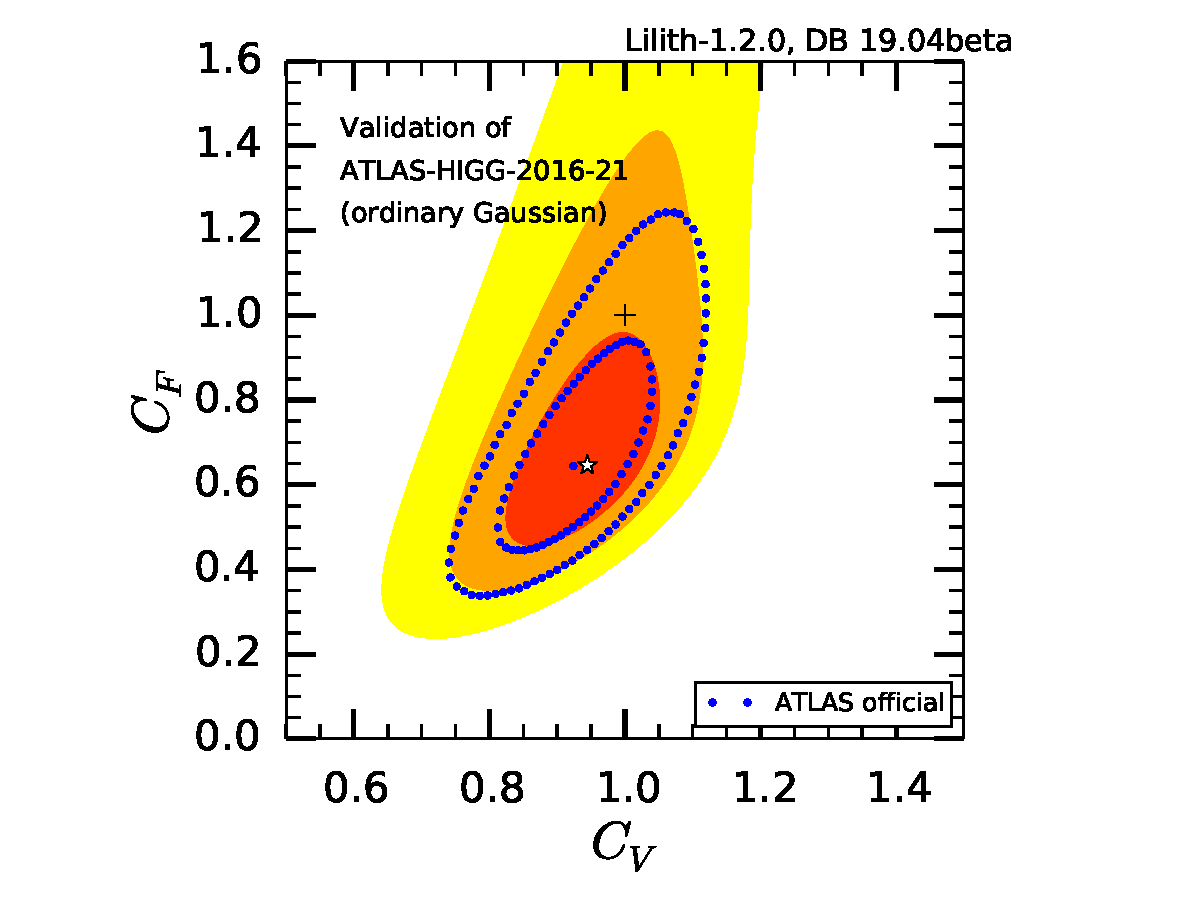
\includegraphics[width=0.43\textwidth]{validation/ATLAS/HIGG-2016-21-CVCF-Gaussian.pdf}%
%\hspace*{-12mm}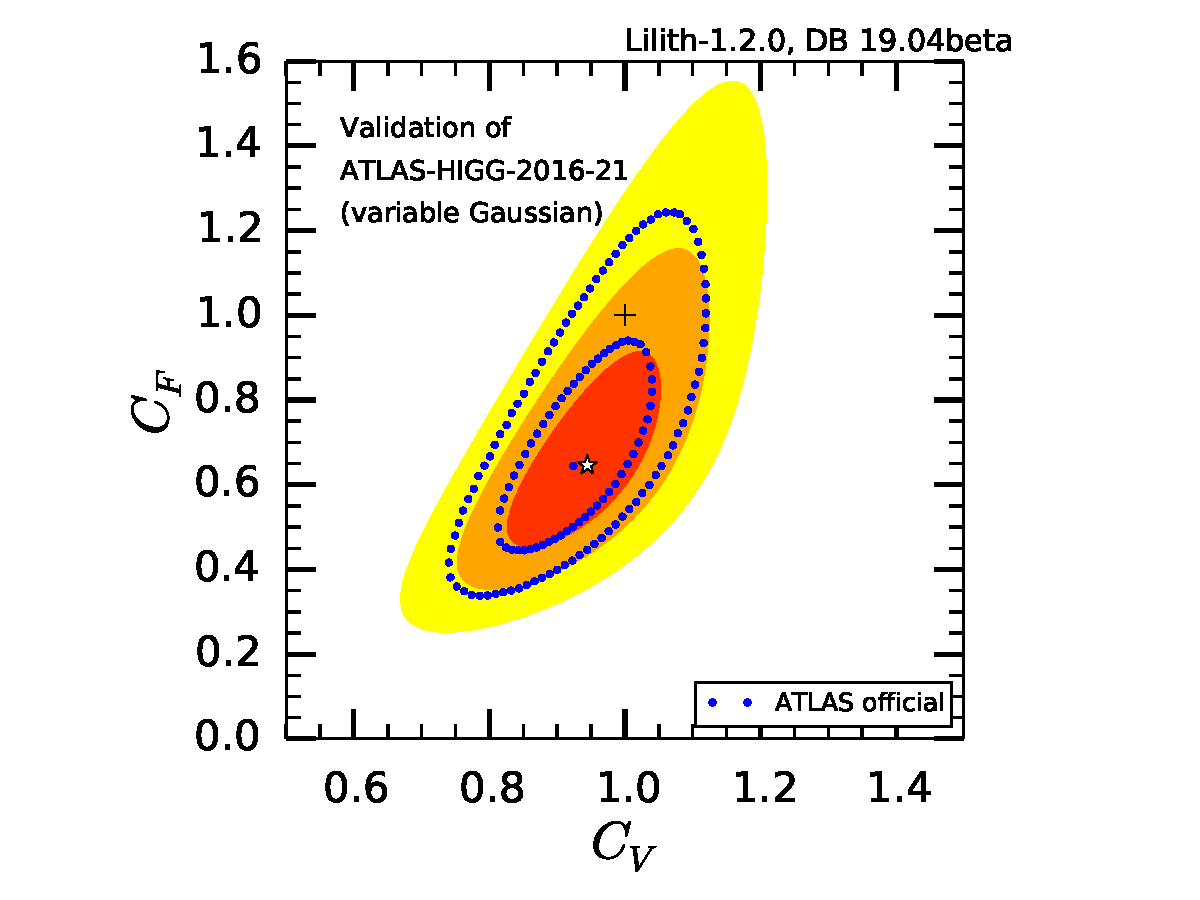
\includegraphics[width=0.43\textwidth]{validation/ATLAS/HIGG-2016-21-CVCF-GaussianV2.pdf}%
%\hspace*{-12mm}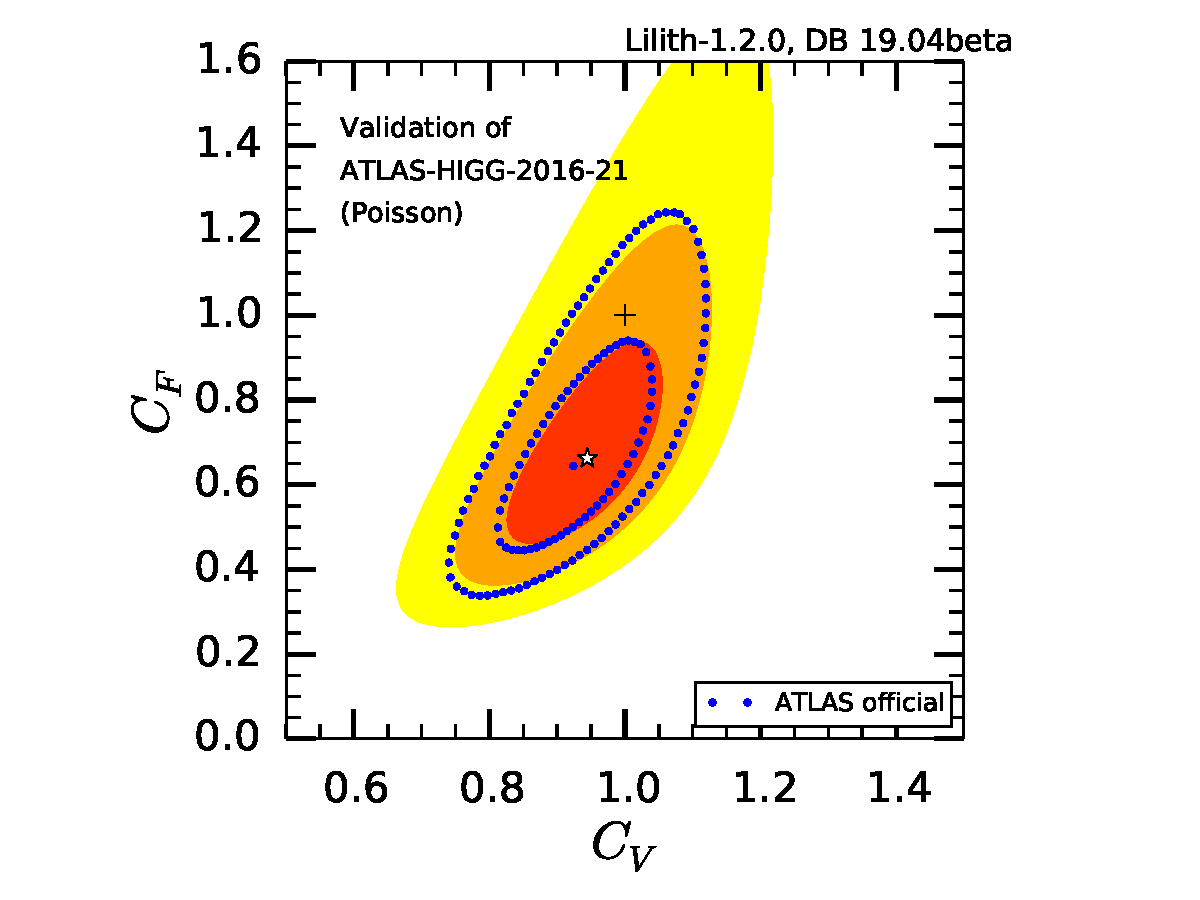
\includegraphics[width=0.43\textwidth]{validation/ATLAS/HIGG-2016-21-CVCF-Poisson.pdf} 
%\caption{Fits of $C_V$ vs.\ $C_F$ using data from the ATLAS $H\to\gamma\gamma$ measurement~\cite{Aaboud:2018xdt}; 
%the signal strength measurements are implemented, from left to right, as ordinary Gaussian, variable Gaussian and Poisson likelihoods.}
%\label{validation_atlas_gamgam}
%\end{figure}
 
\subsubsection*{\boldmath $H\to ZZ^*\to 4l$: HIGG-2016-22}


\subsubsection*{\boldmath $H\to WW^*\to 2l2\nu$: HIGG-2016-07}

\subsubsection*{\boldmath $H\to \tau\tau$: HIGG-2017-07}

\subsubsection*{\boldmath $H\to b\bar b$: HIGG-2016-29 (VH) and HIGG-2016-30 (VBF)}

HIGG-2016-29 provides in Fig.~5 the $1\sigma$ intervals for the $ZH$ and $WH$  production modes. 



\subsubsection*{\boldmath $ttH$}

\subsubsection*{\boldmath $H\to inv$: HIGG-2016-28}

Results from the search for invisibly decaying Higgs bosons produced in association with a $Z$ boson are presented in \cite{Aaboud:2017bja}. Assuming the Standard Model $ZH$ production cross-section, an observed (expected) upper limit of 67\% (39\%) at the 95\% confidence level is set on BR$(H\to inv)$ for $m_H= 125$~GeV. We use $1-{\rm CLs}$ as function BR$(H\to inv)$ extracted from auxiliary Figure~1c on the analysis' webpage. 



%-----------------------------------------------------------------------------------------------
\subsection{CMS Run~2 results for 36~fb$^{-1}$}
%-----------------------------------------------------------------------------------------------

The CMS Run~2 results included in this release are summarised in Table~\ref{tab:CMSresults} and explained in more detail below.

\begin{table}[h]\centering
\begin{tabular}{l | ccccccc}
mode & $\gamma\gamma$ & $ZZ$ & $WW$ & $\tau\tau$ & $b\bar b$ & $\mu\mu$ & inv. \\
\hline
ggH & \cite{Sirunyan:2018koj} & \cite{Sirunyan:2018koj} & \cite{Sirunyan:2018koj} & \cite{Sirunyan:2018koj} & \cite{Sirunyan:2018koj} & \cite{Sirunyan:2018koj} & \cite{Sirunyan:2018owy} \\
VBF &  \cite{Sirunyan:2018koj} & \cite{Sirunyan:2018koj} & \cite{Sirunyan:2018koj} & \cite{Sirunyan:2018koj} &-- & \cite{Sirunyan:2018koj} & \cite{Sirunyan:2018owy} \\
WH &  \cite{Sirunyan:2018koj} & \cite{Sirunyan:2018koj} & \cite{Sirunyan:2018koj} & \cite{Sirunyan:2018cpi} & \cite{Sirunyan:2018koj} & -- & \cite{Sirunyan:2018owy} \\
ZH & \cite{Sirunyan:2018koj} & \cite{Sirunyan:2018koj} & \cite{Sirunyan:2018koj} & \cite{Sirunyan:2018cpi} & \cite{Sirunyan:2018koj} & -- & \cite{Sirunyan:2018owy} \\
ttH & \cite{Sirunyan:2018koj} & \cite{Sirunyan:2018koj} & \cite{Sirunyan:2018koj} & \cite{Sirunyan:2018koj} & \cite{Sirunyan:2018koj} & -- & -- \\
\end{tabular}
\caption{Overview of CMS Run~2 results included in this release. Note that we use the full $24\times 24$ correlation matrix 
for the signal strengths for each production and decay mode combination provided in \cite{Sirunyan:2018koj}.}
\label{tab:CMSresults}
\end{table}



{\bf\boldmath Combined measurements (HIG-17-031):} 
CMS presented in \cite{Sirunyan:2018koj} a combination of the individual measurements for the 
$H\to \gamma\gamma$~\cite{Sirunyan:2018ouh}, $ZZ$~\cite{Sirunyan:2017exp}, $WW$~\cite{Sirunyan:2018egh}, 
$\tau\tau$~\cite{Sirunyan:2017khh}, $b\bar b$~\cite{Sirunyan:2017elk,Sirunyan:2017dgc} and $\mu\mu$~\cite{Sirunyan:2018hbu} 
decay modes as well as the $t\bar tH$ analyses~\cite{Sirunyan:2018shy,Sirunyan:2018mvw,Sirunyan:2018ygk}. 
We use the best fit values and uncertainties for the signal strengths for each production %(ggH, VBF, WH, ZH, ttH) 
and decay  %($\gamma\gamma$, $ZZ$, $WW$, $\tau\tau$, $b\bar b$, $\mu\mu$) 
mode combination presented in Table~3 of \cite{Sirunyan:2018koj} together with the $24\times 24$ (!) correlation matrix 
provided in `Additional Figure~1' on the analysis webpage. As shown in Fig.~\ref{fig:validation_cms_combination}, 
this allows to reproduce well the coupling fits of the CMS paper.\\

\begin{figure}[h!]\centering
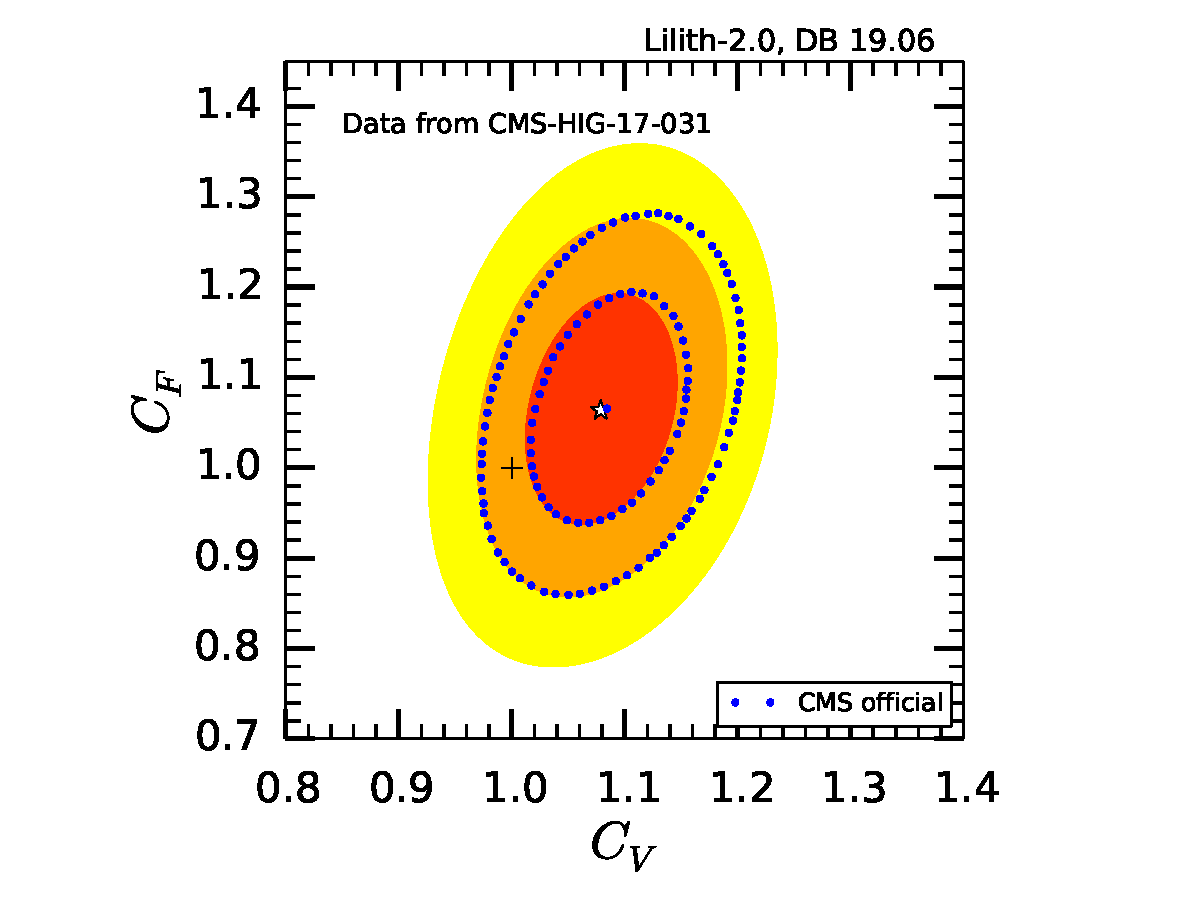
\includegraphics[width=0.5\textwidth]{validation/CMS/HIG-17-031-CVCF.pdf}
%\hspace*{-12mm}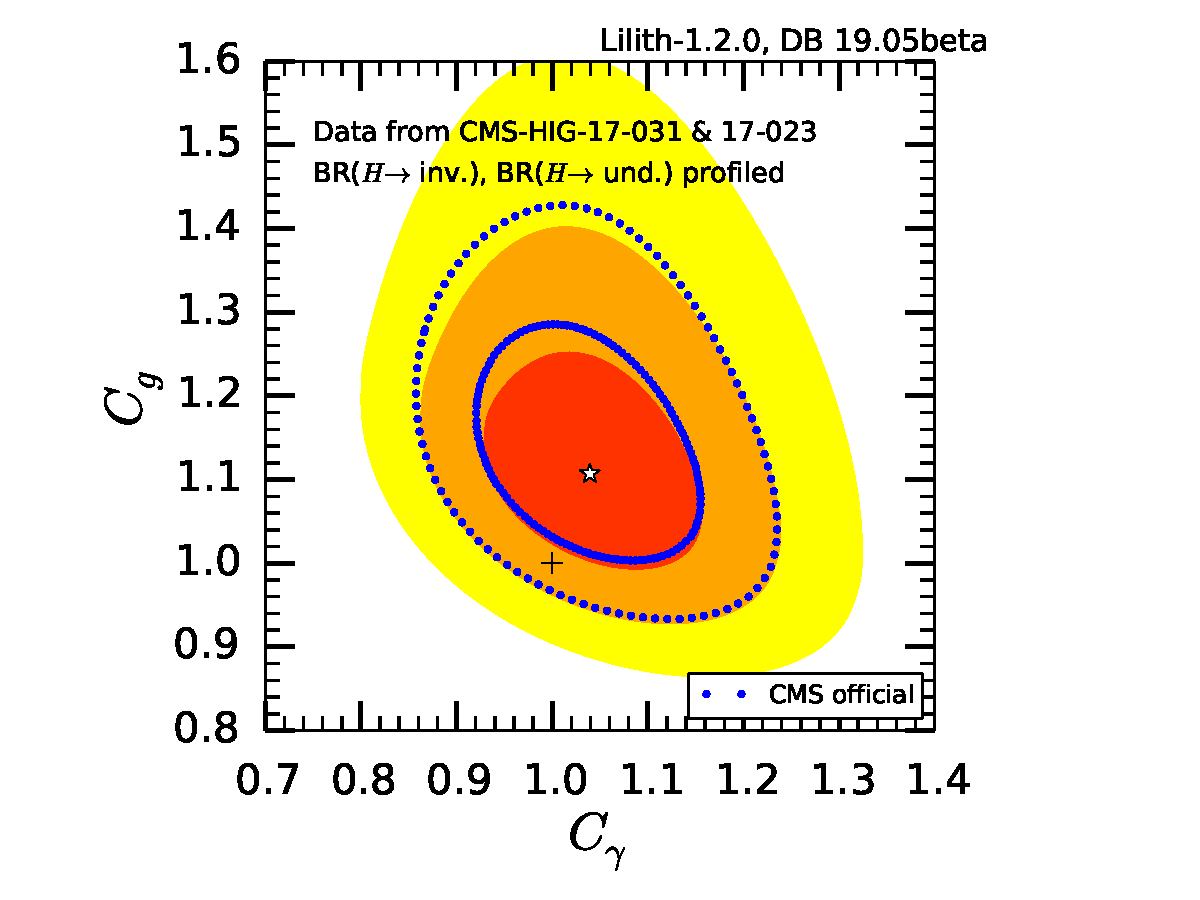
\includegraphics[width=0.43\textwidth]{validation/CMS/HIG-17-031-CgCGa_BRinvBRund_profiled.pdf}%
%\hspace*{-12mm}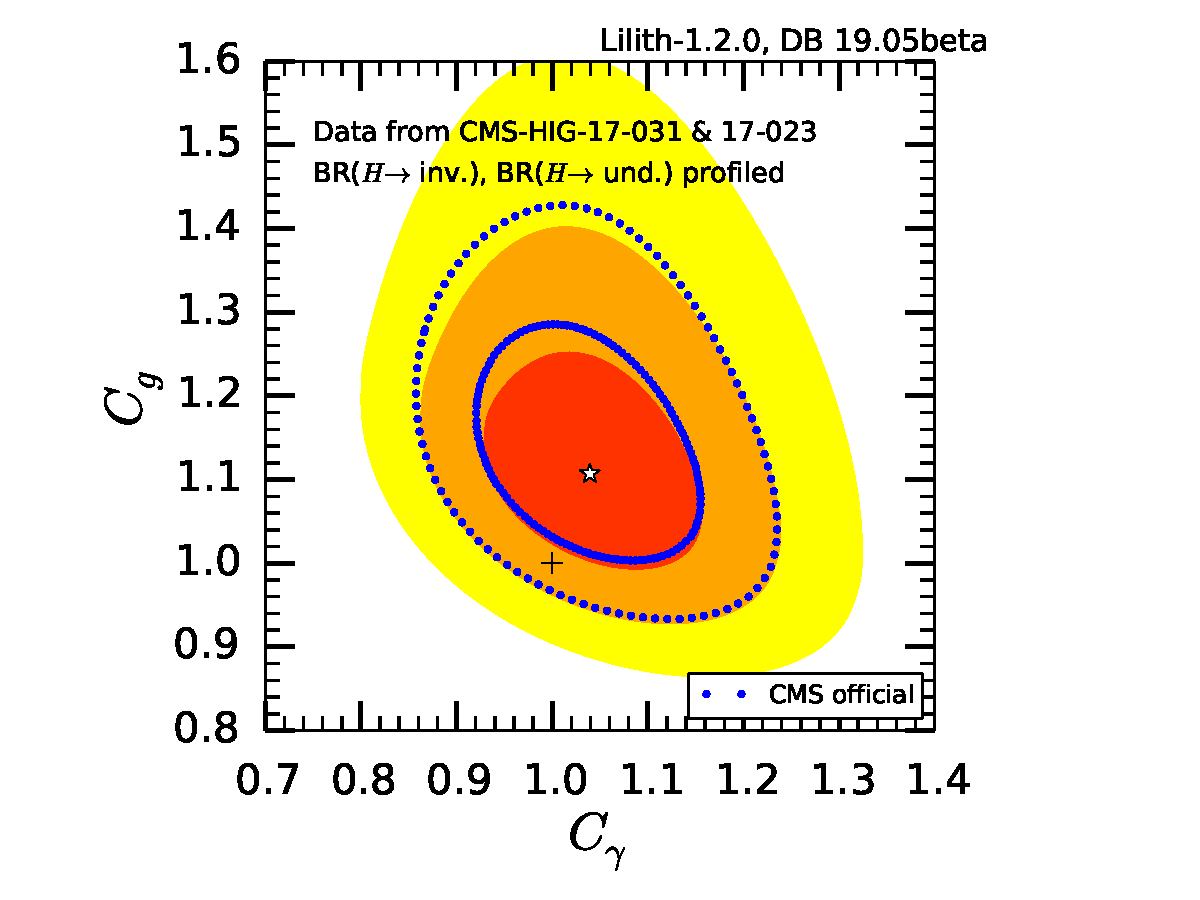
\includegraphics[width=0.43\textwidth]{validation/CMS/HIG-17-031-CgCGa_BRinvBRund_profiled.pdf} 
\caption{Fit of $C_F$ vs.\ $C_V$ using best fit values and uncertainties for the signal strengths for each production (ggH, VBF, WH, ZH, ttH) 
and decay ($\gamma\gamma$, $ZZ$, $WW$, $\tau\tau$, $b\bar b$, $\mu\mu$) mode combination together with the 
$24\times 24$ correlation matrix from the CMS combination paper~\cite{Sirunyan:2018koj}.}
\label{fig:validation_cms_combination}
\end{figure}


{\bf\boldmath $VH$, $H\to\tau\tau$ (HIG-18-007)}: The above data from \cite{Sirunyan:2018koj} is supplemented by the results 
for the $\tau\tau$ decay mode from the $WH$ and $ZH$ targeted analysis \cite{Sirunyan:2018cpi}. These are implemented in the 
form of 1D intervals for $\mu(ZH,\;H\to\tau\tau)$ and $\mu(WH,\;H\to\tau\tau)$ taken from Fig.~6 of \cite{Sirunyan:2018cpi}. \\

{\bf\boldmath $H\to$~invisible (HIG-17-023)}: 
In \cite{Sirunyan:2018owy}, CMS performed a search for invisible decays of a Higgs boson produced through vector boson fusion. 
We use the profile likelihood ratios for the qqH-tag, Z(ll)H-, V(qq')H- and ggH-tag categories extracted 
from their Fig.~8b together with the relative contributions from the different Higgs production mechanisms  
given in Table~6 of that paper. This assumes that the relative signal contributions stay roughly the same as for 
SM production cross sections. For validation, we reproduce in Fig.~\ref{fig:validation_cms_inv}
 the $C_g$ vs.\ $C_\gamma$ fit of \cite{Sirunyan:2018koj}, where the branching ratios of invisible and undetected decays 
are treated as free parameters.\footnote{The profiling was done with Minuit. Since Minuit does not allow conditional limits, like 
${\rm BR}(H\to {\rm inv.})+{\rm BR}(H\to {\rm undetected})<1$, we demanded that both BR$(H\to {\rm inv.})$ and BR$(H\to {\rm undetected})$ 
stay below 50\%. This explains in part the small difference to the official CMS result.}

\begin{figure}[h!]\centering
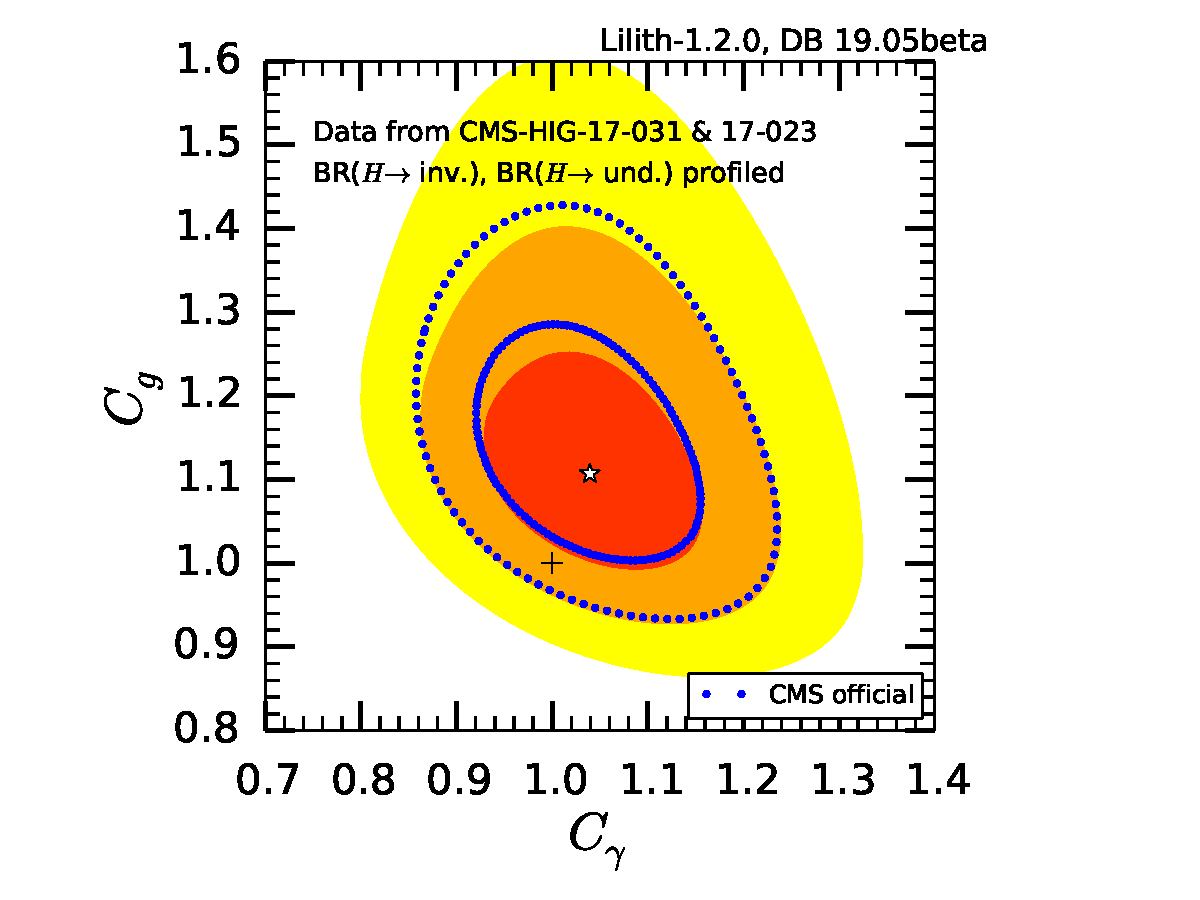
\includegraphics[width=0.5\textwidth]{validation/CMS/HIG-17-031-CgCGa_BRinvBRund_profiled.pdf}
%\hspace*{-12mm}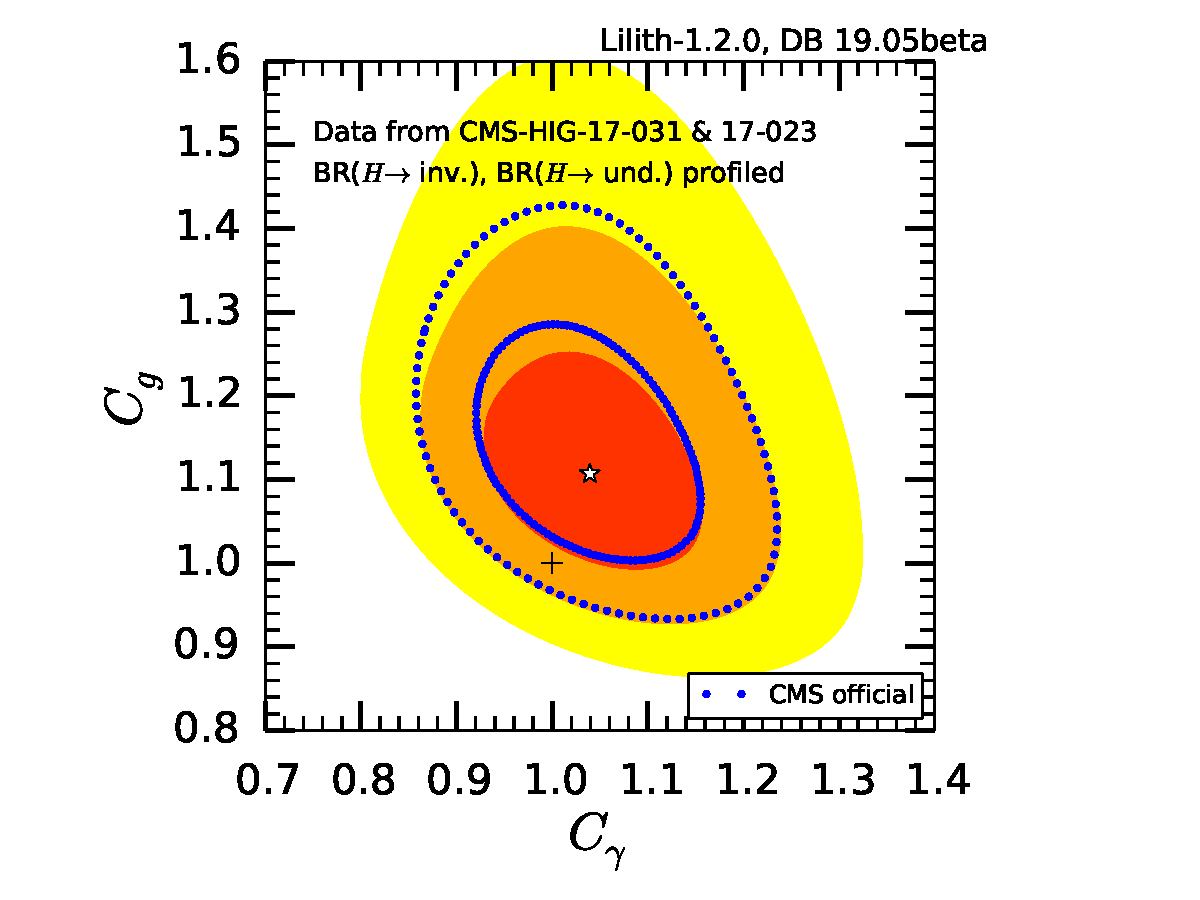
\includegraphics[width=0.43\textwidth]{validation/CMS/HIG-17-031-CgCGa_BRinvBRund_profiled.pdf}%
%\hspace*{-12mm}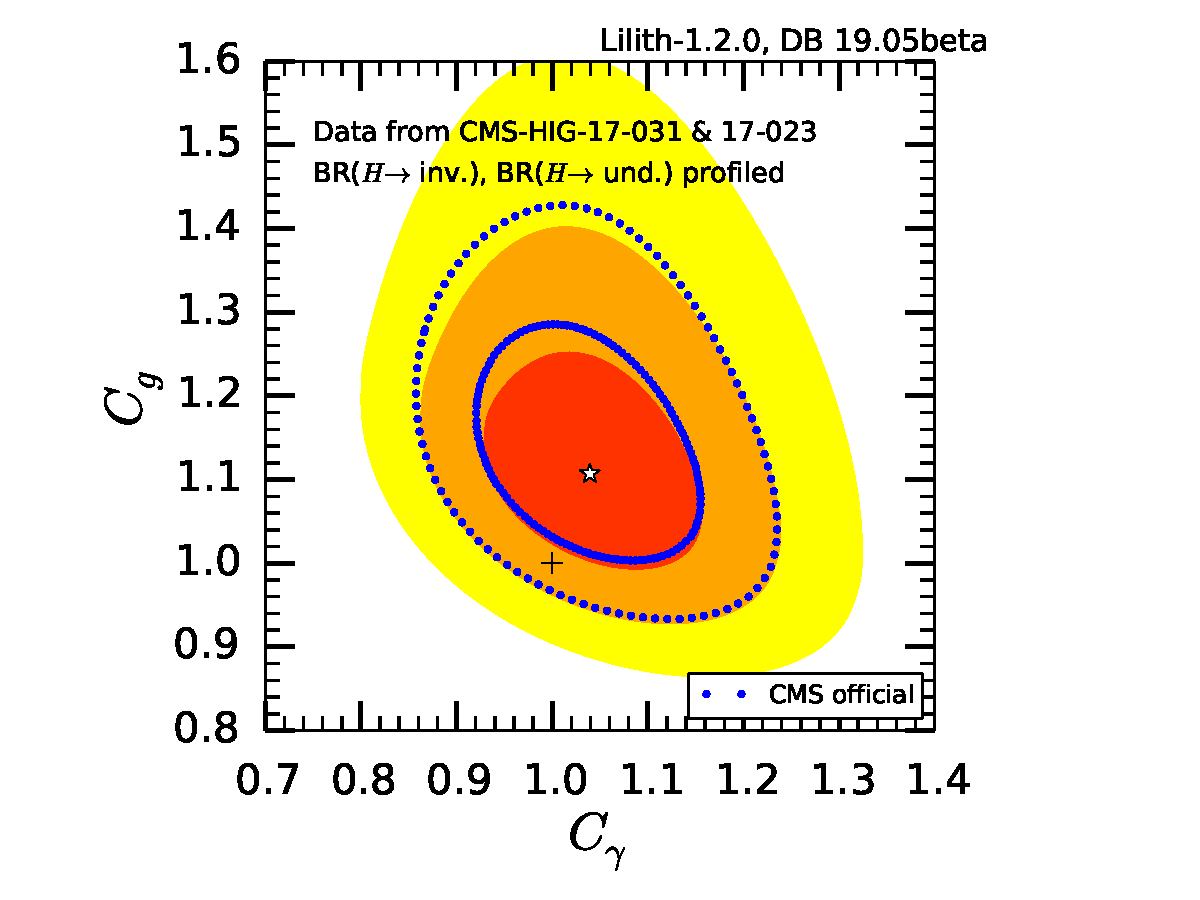
\includegraphics[width=0.43\textwidth]{validation/CMS/HIG-17-031-CgCGa_BRinvBRund_profiled.pdf} 
\caption{Fit of $C_g$ vs.\ $C_\gamma$ using the data from the combined CMS measurement~\cite{Sirunyan:2018koj} and the 
search for invisible decays of a Higgs boson~\cite{Sirunyan:2018owy}. The branching ratios of invisible and undetected decays 
are treated as free parameters in the fit.}
\label{fig:validation_cms_inv}
\end{figure}




%===================================================================================
\section{Status of Higgs coupling fits}
%===================================================================================


%===================================================================================
\section{Conclusion}
%===================================================================================
 must include a conclusion.

%===================================================================================
\section*{Acknowledgements}
%===================================================================================

S.K.~thanks W.~Adam, R.~Sch\"ofbeck, W.~Waltenberger and N.~Wardle for helpful discussions. 

%\paragraph{Author contributions}
%This is optional. If desired, contributions should be succinctly described in a single short paragraph, using author initials.

%\paragraph{Funding information}
%Authors are required to provide funding information, including relevant agencies and grant numbers with linked author's initials. Correctly-provided data will be linked to funders listed in the \href{https://www.crossref.org/services/funder-registry/}{\sf Fundref registry}.
This work was supported by the IN2P3 theory project 
``LHC-itools: methods and tools for the interpretation of the LHC Run~2 results for new physics''. 
D.T.N.\ thanks the LPSC Grenoble for hospitality and financial support for a research visit within the LHC-itools project. 
L.T.Q.\ thanks the ICISE ...


%===================================================================================
\begin{appendix}
%===================================================================================

\section{Overview of XML data files}

\section{Implementation of 2D Poisson likelihood with correlation}


\end{appendix}


%===================================================================================
% References
%===================================================================================

% \bibliographystyle{SciPost_bibstyle} % Include this style file here only if you are not using our template
\bibliography{references.bib}

\nolinenumbers

\end{document}
